\subsection*{\hypertarget{combat}{Combate}}
\addcontentsline{toc}{subsection}{Combate}
%
"Basta de charla. Es hora de luchar como hombres.\newline Y mujeres. Y mujeres que se visten como hombres".\\
\indent -- Gilgamesh 
%
\begin{center} \includegraphics[width=1\columnwidth]{./art/images/ff13-2.png} \end{center}
%
\vspace{0.5cm}
%
El combate se lleva a cabo en una serie de \textbf{turnos} (\textbf{t}) que representan 10 segundos en el tiempo de la partida cada uno.
Cada participante tiene un \textbf{turno }por ronda según el orden determinado a través de una \mbox{\textbf{tirada de iniciativa }}al principio de cada batalla. Cada combatiente tira 2d y el orden se define por los resultados de esas tiradas en orden descendente. El DJ define los empates y una vez que se ha definido, el orden de los turnos no cambia hasta el final de la batalla. Durante tu turno puedes, en cualquier orden, mover una distancia igual a tu AGI+1 y realizar una acción.
%
\vfill
%
\subsubsection*{Atributos}
La pericia en combate está determinada por los siguientes 7 atributos numéricos. Cada vez que un cálculo resulte en un valor no entero, el resultado siempre se redondea hacia abajo.
%
\begin{description}[leftmargin=*]
	\item[\large\color{accent} \raisebox{-.2\height}{\includegraphics[height=0.9\baselineskip]{./art/icons/hp.png}} Puntos de vida (PV): ] representan tu salud. Tienes una cantidad máxima de PV y si tus PV llegan a 0, quedas inconsciente. \item[\large\color{accent} \raisebox{-.2\height}{\includegraphics[height=0.9\baselineskip]{./art/icons/mp.png}} Puntos de Maná (PM): ] son un recurso necesario para utilizar habilidades como la Magia y las Técnicas. Al igual que los PV, tienes un número máximo y un número actual de PM. \item[\large\color{accent} \raisebox{-.2\height}{\includegraphics[height=0.9\baselineskip]{./art/icons/str.png}} Fuerza (FUE):] aumenta el daño provocado por tus ataques físicos. \item[\large\color{accent} \raisebox{-.2\height}{\includegraphics[height=0.9\baselineskip]{./art/icons/def.png}} Defensa (DEF):] aumenta tu resistencia contra ataques físicos. \item[\large\color{accent} \raisebox{-.2\height}{\includegraphics[height=0.9\baselineskip]{./art/icons/mag.png}} Magia (MAG):] aumenta la potencia de tus hechizos de daño y curación. \item[\large\color{accent} \raisebox{-.2\height}{\includegraphics[height=0.9\baselineskip]{./art/icons/res.png}} Resistencia (RES:)] aumenta tu resistencia contra ataques mágicos. \item[\large\color{accent} \raisebox{-.2\height}{\includegraphics[height=0.9\baselineskip]{./art/icons/mov.png}} Agilidad (AGI):] te permite evadir los ataques físicos y determinar con qué rapidez puedes moverte.
\end{description}

\vfill

\subsubsection*{\hypertarget{action}{Acciones}}
A continuación se muestra una lista de acciones de combate, pero el DJ puede permitir cualquier otra acción que pueda completarse en un solo turno:
\begin{description}[leftmargin=*]	
	\item[\large\color{accent} \raisebox{-.2\height}{\includegraphics[height=0.9\baselineskip]{./art/icons/attack.png}} \textbf{Ataque}:] Atacas a un enemigo con tu arma. Tu enemigo puede evadir pasando una \textbf{tirada de evasión} con DC 12 menos su AGI. Si falla la tirada, se reducen los PV del objetivo por el daño de tu arma más su FUE. Si quien intenta evadir el ataque saca un 2, logras hacerle \mbox{\textbf{daño crítico}}, lo que duplica el daño normal. Si saca un 12, no solo fallas el ataque, sino que tu objetivo realiza una acción de ataque que no puedes evadir. \item[\large\color{accent}  \raisebox{-.2\height}{\includegraphics[height=0.9\baselineskip]{./art/icons/magic.png}} \textbf{Magia}:] Lanzas un hechizo gastando PM. Debes elegir un objetivo dentro del alcance del hechizo y \mbox{\textbf{concentrarte}} por un tiempo establecido. Mientras te concentras, no puedes realizar acciones ni evadir ataques. Una vez que el tiempo de concentración termina, el efecto del hechizo se produce en el objetivo \textbf{antes de tu turno }y no se puede evadir (incluso si el objetivo no está en el alcance del hechizo). Si el hechizo provoca daño o restaura PV, suma tu MAG al total. La descripción de cada hechizo tiene información sobre su tiempo de preparación, coste de PM, objetivo, alcance y efecto. \item[\large\color{accent}  \raisebox{-.2\height}{\includegraphics[height=0.9\baselineskip]{./art/icons/tech.png}} \textbf{Técnicas}:] Utilizas una habilidad no mágica. Las técnicas se utilizan del mismo modo que la magia, pero tus atributos no aumentan el daño. \item[\large\color{accent}  \raisebox{-.2\height}{\includegraphics[height=0.9\baselineskip]{./art/icons/defend.png}} \textbf{Defender}:] Todo el daño que recibas de \hyperlink{action}{Ataques} se reducirá a la mitad hasta tu próximo turno. \item[\large\color{accent}  \raisebox{-.2\height}{\includegraphics[height=0.9\baselineskip]{./art/icons/item.png}} \textbf{Objeto}:] Utiliza un objeto de tu inventario sobre ti o sobre alguien a 1u de distancia. 
\end{description} 
\subsubsection*{\hypertarget{sabilities}{Habilidades especiales}}
Además de la Magia y las Técnicas, los personajes también pueden aprender las siguientes habilidades especiales:
%
\begin{description}[leftmargin=*]
	\item[\large\color{accent} \raisebox{-.2\height}{\includegraphics[width=\baselineskip]{./art/icons/passive.png}} \textbf{Pasivas}:] Efectos que están permanentemente activados. \item[\large\color{accent} \raisebox{-.2\height}{\includegraphics[width=\baselineskip]{./art/icons/react.png}} \textbf{Reacción}:] Te permite realizar ciertas acciones durante el turno de alguien más si se dan ciertas circunstancias específicas.
\end{description}
%
\vspace{0.2cm}
%
\example{Combate}
{
 Squall (\textcolor{blue}{DEF:4}, \textcolor{ForestGreen}{AGI:2}, \textcolor{Sepia}{RES:1}) y Seifer (\textcolor{red}{FUE:6}, \textcolor{Magenta}{MAG:2}) se baten a duelo. Ambos están utilizando un sable-pistola (Daño:\textcolor{Plum}{1d}). Tiran 2d por iniciativa: Squall y Seifer sacan 9 y 10 respectivamente, por lo que Seifer tiene el primer turno. Comienza preparando "Piro" (Daño:\textcolor{orange}{2d}, Tiempo:1t). Gasta 4 PM, elige a Squall como objetivo y se concentra. Es el turno de Squall, quien elige Defender. Es turno de Seifer otra vez, por lo que Piro surte efecto y Squall recibe \mbox{\textcolor{orange}{2d}+\textcolor{Magenta}{2}-\textcolor{Sepia}{1}} de daño. Aún es turno de Seifer, así que también Ataca. Squall podría evadir el ataque pasando una tirada con \mbox{DC 12-\textcolor{ForestGreen}{2}}. Sin embargo, saca un 2, así que no solo falla en su intento de evadir, sino que sufre daño crítico. Seifer lo golpea justo por encima de la nariz con el sable, causando \mbox{\textcolor{Plum}{1d}+\textcolor{red}{6}-\textcolor{blue}{4} }
 de daño (Defender y daño crítico se cancelan entre sí) y deja una cicatriz.
}
\subsubsection*{Tipos de Daño} 
Todos los daños sufridos pertenecen a uno de los siguientes tipos básicos:
%
\begin{description}[leftmargin=*]
 \item[\accf{Físico}:] los daños provocados por Ataques y Técnicas son generalmente físicos. Cuando recibas daño físico, resta tu DEF del total.
  
 \item[\accf{Mágico}:] los daños provocados por Magia y Objetos generalmente son mágicos. Cuando recibas daño mágico, resta tu RES del total.
\end{description}
%
\noindent
Además, los daños pueden ser de tipo de elemental, por ejemplo, debido al arma o el hechizo utilizado. Los combatientes pueden tener \textbf{Debilidades }o \textbf{Resistencias }contra estos tipos. Cuando son resistentes, solo sufren la mitad del daño habitual y, cuando son débiles, sufren el doble del daño habitual. 
%
\vspace{0.1cm}
%
\begin{tcolorbox}[colback=white, left=1pt,top=0pt,right=1pt,bottom=0pt,colframe=accent,tabularx={@{\hspace{-0.2cm}}cp{0.45\columnwidth}|p{0.45\columnwidth}},sharp corners=south, title={\begin{center} \textbf{Tipos de Daño Elemental} \end{center}}] 
	& \textbf{Fuego} \hspace*{\fill} \raisebox{-.4\height}{\includegraphics[width=0.05\columnwidth]{./art/icons/fire.png}} &
 \textbf{Hielo} \hspace*{\fill} \raisebox{-.4\height}{\includegraphics[width=0.05\columnwidth]{./art/icons/ice.png}}  \vspace{0.1cm} \\
	\hline & \textbf{Electricidad} \hspace*{\fill} \raisebox{-.4\height}{\includegraphics[width=0.05\columnwidth]{./art/icons/lightning.png}}  &
 \textbf{Agua} \hspace*{\fill} \raisebox{-.4\height}{\includegraphics[width=0.05\columnwidth]{./art/icons/water.png}} \vspace{0.1cm} \\ 
	\hline & \textbf{Viento} \hspace*{\fill} \raisebox{-.4\height}{\includegraphics[width=0.05\columnwidth]{./art/icons/wind.png}} &
 \textbf{Tierra} \hspace*{\fill} \raisebox{-.4\height}{\includegraphics[width=0.05\columnwidth]{./art/icons/earth.png}} \vspace{0.1cm} \\
	\hline & \textbf{Sagrado} \hspace*{\fill} \raisebox{-.4\height}{\includegraphics[width=0.05\columnwidth]{./art/icons/holy.png}}  &
 \textbf{Oscuro} \hspace*{\fill} \raisebox{-.4\height}{\includegraphics[width=0.05\columnwidth]{./art/icons/dark.png}} \vspace{0.1cm} \\
\end{tcolorbox}

\subsubsection*{Distancias}
Las \textbf{Unidades} (abreviado \textbf{u}) son la base para medir la distancia (1u es aproximadamente 1m). Generalmente, los personajes ocupan un círculo de 1u de diámetro en la vista superior. A menudo se utilizan los siguientes términos para describir las distancias de los efectos:
%
\begin{description}[leftmargin=*]
 \item[\accf{Alcance}:] la máxima distancia entre el centro del lanzador y el centro del efecto. Un efecto con alcance \textbf{Tú} está centrado en el lanzador y uno con alcance \textbf{Arma} tiene el mismo alcance que el arma empuñada. \item[\accf{AdE}:] es el área de efecto máxima de una habilidad desde su centro. A menos que se indique lo contrario, todos los que estén dentro del área quedan afectados parcial o totalmente, incluidos los aliados. Un efecto con AdE \textbf{Individual} afecta solo a una entidad.
\end{description}
%
% Range / Distance Illustration	
\begin{figure}[h]
		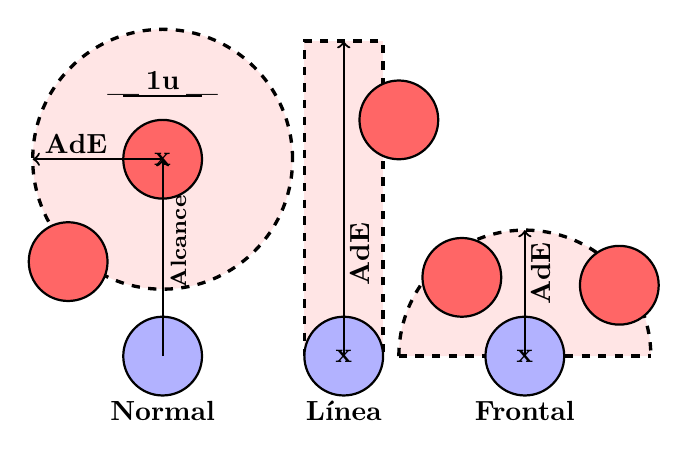
\begin{tikzpicture}[]
		\tikzstyle{test}=[thick, draw, circle, align=center]					
		%Normal
		\node[fill=blue!30!white, test,minimum size = 1cm](caster)at (0,0) {};
		\node[](t2)at (0,-0.7) {\bf Normal};
		\node[fill=red!10!white, test, very thick, dashed ,minimum size = 3.3cm](tarea)at (0,2.5) {};
		\node[fill=red!60!white, test,minimum size = 1cm](target)at (0,2.5) {};
		\node[fill=red!60!white, test,minimum size = 1cm](target)at (-1.2,1.2) {};
		\draw[thick, ->](0,0) -- node[] {}(0,2.5);
		\draw[thick, ->](0,2.5) -- node[] {}(-1.65,2.5);
		\node[rotate=90](t1)at (0.2,1.45) {\bf \footnotesize Alcance};
		\node[](t2)at (-1.1,2.7) {\bf AdE};
		\node[](t3)at (0,2.5) {\bf x};
		\node[](fi)at (-0.5,3.3) {\bf |};
		\node[](se)at (0.5,3.3) {\bf |};
		\draw[thick, -](0.5,3.3) -- node[] {}(-0.5,3.3);
		\node[](sca)at (0,3.5) {\bf 1u};		
		%Line
		\node[draw, fill=red!10!white, rectangle, very thick, dashed ,minimum height = 4cm, minimum width=1cm](tarea)at (2.3,2) {};
		\node[fill=blue!30!white, test,minimum size = 1cm](caster)at (2.3,0) {};
		\node[](t2)at (2.3,-0.7) {\bf Línea};
		\node[fill=red!60!white, test,minimum size = 1cm](target)at (3,3) {};
		\draw[thick, ->](2.3,0) -- node[] {}(2.3,4);
		\node[rotate=90](t1)at (2.5,1.3) {\bf AdE};
		\node[](t3)at (2.3,0) {\bf x};		
		%Front
		\draw[fill=red!10!white, test, very thick, dashed] (3,0) arc (180:0:1.6cm);
		\draw[dashed, very thick, -](3,0) -- node[] {}(6.2,0);
		\node[fill=blue!30!white, test,minimum size = 1cm](caster)at (4.6,0) {};
		\node[](t2)at (4.6,-0.7) {\bf Frontal};
		\draw[thick, ->](4.6,0) -- node[] {}(4.6,1.6);
		\node[rotate=90](t1)at (4.8,1.05) {\bf AdE};
		\node[fill=red!60!white, test,minimum size = 1cm](target)at (3.8,1) {};
		\node[fill=red!60!white, test,minimum size = 1cm](target)at (5.8,0.9) {};
		\node[](t3)at (4.6,0) {\bf x};
		\end{tikzpicture}
\end{figure}
%
\noindent
La ilustración anterior muestra el uso de un efecto a distancia en una situación normal y con las dos formas de AdE especiales: \textbf{Línea} y \textbf{Frontal}. En situaciones en las que no puedas medir las distancias con precisión, también puedes utilizar las siguientes descripciones para dar una estimación aproximada:
%
\pagebreak
%
\begin{description}[leftmargin=*]
 \item[\accf{Adyacente}:] aproximadamente una distancia de 1u o menos. \item[\accf{Cerca}:] aproximadamente una distancia de entre 1u y 3u. \item[\accf{Media distancia}:] aproximadamente una distancia de entre 3u y 6u. \item[\accf{Lejos}:] aproximadamente una distancia de 6u o más.
\end{description}
\subsubsection*{\hypertarget{status}{Estados Alterados}}
Los estados alterados afectan la potencia de combate de forma positiva o negativa durante un período de tiempo. Los combatientes pueden sufrir múltiples estados alterados a la vez, pero aplicar el mismo dos veces solo actualiza su duración. También pueden ser \textbf{Inmunes} a ciertos estados, lo que significa que no tienen ningún efecto. A continuación se muestra una lista de todos los estados alterados.
\begin{description}[leftmargin=*]
	
	\item[\large\color{accent} \raisebox{-.2\height}{\includegraphics[width=\baselineskip]{./art/icons/doom.png}} \textbf{KO}:] Estás inconsciente y se omiten tus turnos. Pasas a estar KO cuando tus PV actuales llegan a 0. Tus PV no pueden aumentarse hasta recuperarte de este estado. La inmunidad contra KO solo te hace inmune frente a los efectos que lo causan cuando estás por encima de 0 PV. \item[\large\color{accent} \raisebox{-.1\height}{\includegraphics[width=\baselineskip]{./art/icons/blind.png}} \textbf{Ceguera}:] Siempre que \hyperlink{action}{Ataques} a un enemigo, éste tiene \hyperlink{check}{Ventaja} en la tirada de evasión. \item[\large\color{accent} \raisebox{-.1\height}{\includegraphics[width=\baselineskip]{./art/icons/blink.png}} \textbf{Reflejos}:] Siempre que recibas un \hyperlink{action}{Ataque}, tienes \hyperlink{check}{Ventaja }en la tirada de evasión. \item[\large\color{accent} \raisebox{-.1\height}{\includegraphics[width=\baselineskip]{./art/icons/debrave.png} 
		\includegraphics[width=\baselineskip]{./art/icons/deprotect.png} \includegraphics[width=\baselineskip]{./art/icons/defaith.png} 
		\includegraphics[width=\baselineskip]{./art/icons/deshell.png}} \textbf{disATR}:] El atributo especificado se reduce en 3 (mínimo 0). Por ejemplo, disMAG reduce MAG. \item[\large\color{accent} \raisebox{-.1\height}{\includegraphics[width=\baselineskip]{./art/icons/bravery.png} 
		\includegraphics[width=\baselineskip]{./art/icons/protect.png} \includegraphics[width=\baselineskip]{./art/icons/faith.png} 
		\includegraphics[width=\baselineskip]{./art/icons/shell.png}} \textbf{aumATR}:] El atributo especificado aumenta en 3. Por ejemplo, aumMAG aumenta MAG. \item[\large\color{accent} \raisebox{-.1\height}{\includegraphics[width=\baselineskip]{./art/icons/immobile.png}} \textbf{Inmóvil}:] No puedes moverte. \item[\large\color{accent} \raisebox{-.1\height}{\includegraphics[width=\baselineskip]{./art/icons/poison.png}} \textbf{Envenenado}:] Recibes daño igual al 10 \% de tus PV máximos al final de cada turno, pero no puedes quedar por debajo de 1 PV debido a este efecto. \item[\large\color{accent} \raisebox{-.1\height}{\includegraphics[width=\baselineskip]{./art/icons/silence.png}} \textbf{Silencio}:] No puedes comenzar a lanzar \hyperlink{action}{Magia} ni utilizar \hyperlink{action}{Técnicas}, pero todavía puedes \hyperlink{action}{Atacar}. \item[\large\color{accent} \raisebox{-.1\height}{\includegraphics[width=\baselineskip]{./art/icons/stop.png}} \textbf{Dormido}:] Se saltean tus turnos, pero te despiertas inmediatamente si recibes daño. \item[\large\color{accent} \raisebox{-.1\height}{\includegraphics[width=\baselineskip]{./art/icons/zombie.png}} \textbf{Zombi}:] Todos los efectos curativos tienen un efecto inverso en ti. La curación reduce tus PV y los efectos que normalmente remueven el KO, lo producen. 
\end{description} 
%
\vspace*{0.25cm}
%
\example{Estados alterados}
{
Noctis y su grupo se enfrentan a un \hyperlink{malboro}{Malboro}. El monstruo los sorprende y utiliza su habilidad Mal Aliento para infligir múltiples estados alterados. Prompto ahora está Dormido y \textcolor{red}{Envenenado}. No puede moverse ni actuar y antes de terminar su turno, pierde \textcolor{red}{3 } PV, porque sus PV máximos son \textcolor{red}{3}7. Noctis sufre Silencio y \textcolor{Plum}{Ceguera}. No puede utilizar habilidades, así que intenta \hyperlink{action}{Atacar} al Malboro. El monstruo (AGI: \textcolor{ForestGreen}{2}) saca [1,6,4] en la tirada de evasión, que apenas pasan la \mbox{DC 12-\textcolor{ForestGreen}{2}} debido a que tiene \textcolor{Plum}{Ventaja}.
}
%
\clearpage








